\lipsum[2-2]

\begin{table}[h]
    \centering
    \caption{Details of Students}
    \renewcommand{\arraystretch}{1.5}
    \begin{tabular}{|c|c|c|}
    \hline
       S.N.  & Name of Student & Addr.\\ \hline
       1  & Janak S. Dhami & KTM\\ \hline
       2  & Janak S. Dhami & KTM\\ \hline
       3  & Janak S. Dhami & KTM\\ \hline
    \end{tabular}
    \label{tab:my_label}
\end{table}

\lipsum[2-2]
\\
\begin{figure}
    \centering
    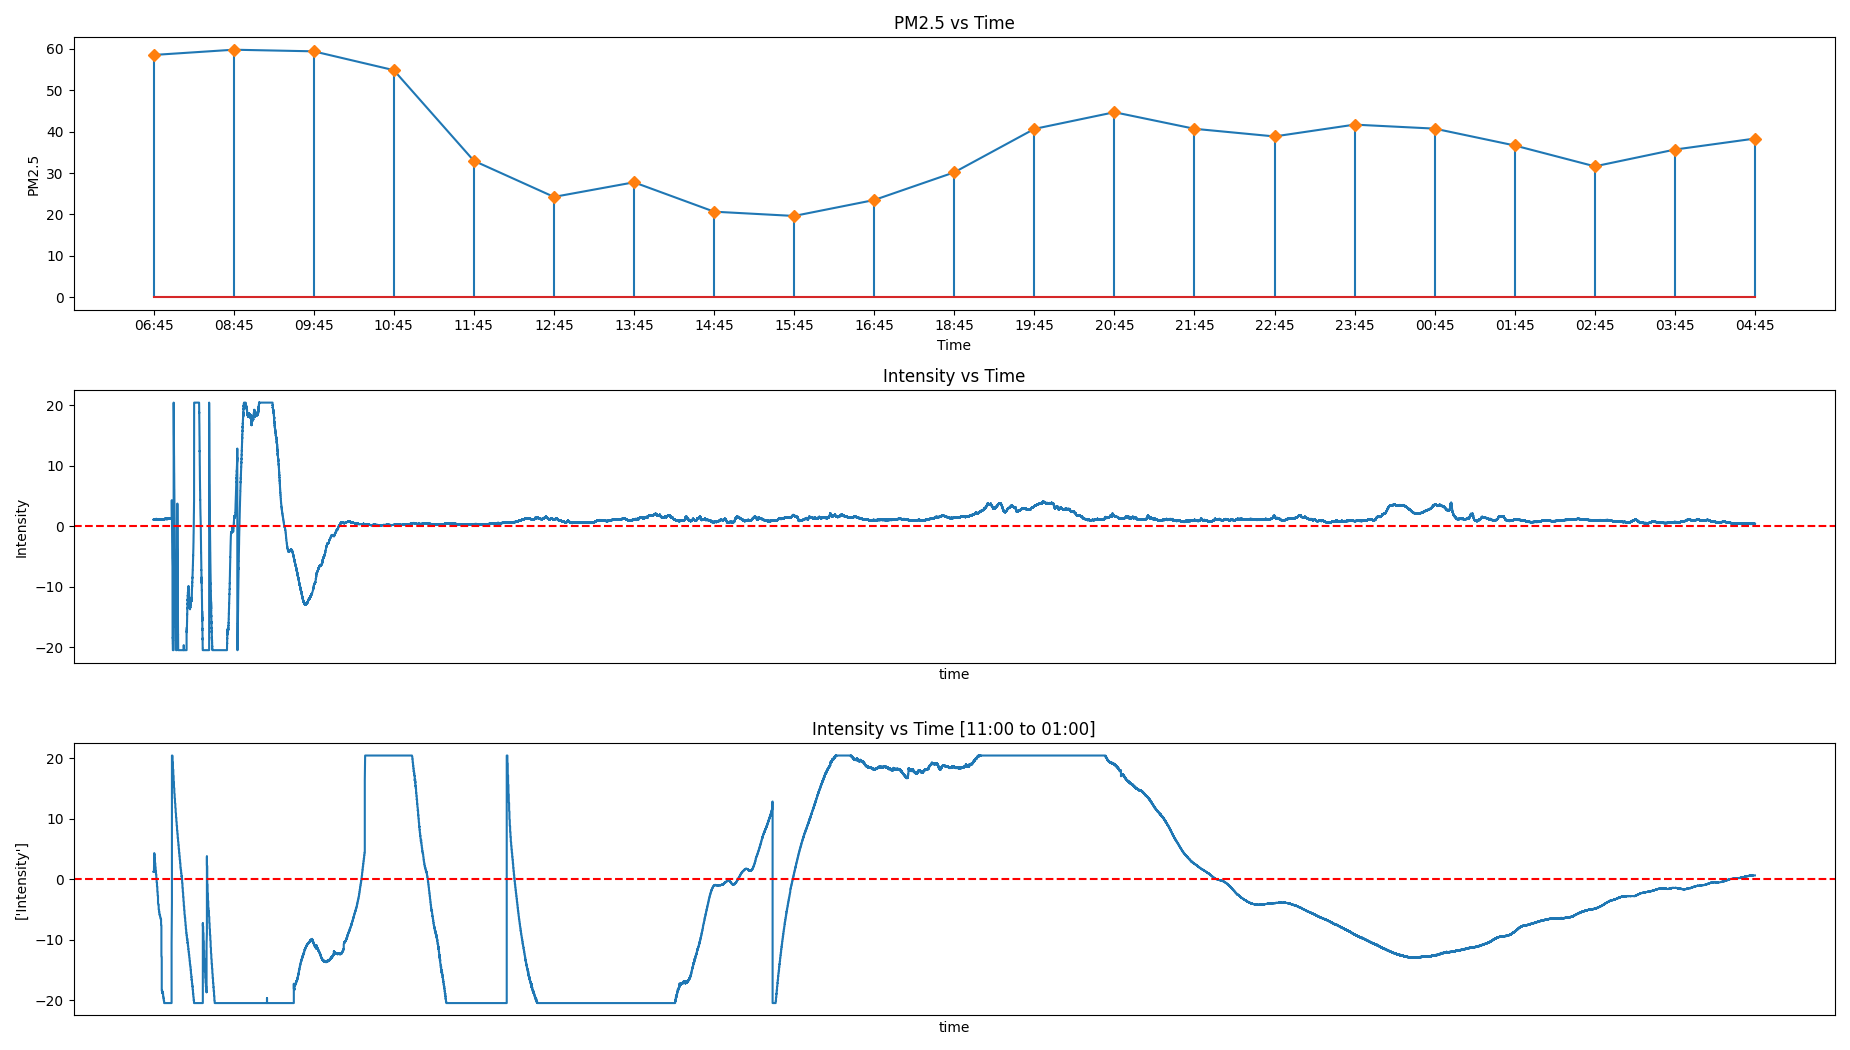
\includegraphics[width=1\linewidth]{images/aq.png}
    \caption{Air Quality in KTM}
    \label{aq}
\end{figure}

\lipsum[1-1]
\begin{enumerate}
    \item The integral $\int_0^1 x^{m-1}(1-x)^{n-1}dx, (m>0, n>0)$ is known as first integral or $\beta$-function.
    \item the integral ....
    \item \[(a+b)^2\]
    \item 
\end{enumerate}
